\hypertarget{loops-and-invariants}{%
\section{Loops and Invariants}\label{loops-and-invariants}}

\hypertarget{invariants}{%
\subsection{Invariants}\label{invariants}}

An assertion I is called an invariant, if a command C doesn't change
anything in regards to the assertion I. -\textgreater{} $\models$ \{ I \} C \{ I
\}

E.g. if you drive through a tunnel by car, you pass an emergency exit
every 250 meters. If you are between two exits and you are driving
forward, you are maximizing the distance to the earlier exit and
minimizing the distance to the next exit, but you don't change the
distance between them. The distance between them is invariant.

\hypertarget{invariants-for-loops}{%
\subsubsection{Invariants for loops}\label{invariants-for-loops}}

\begin{itemize}
\tightlist
\item
  here we need invariants for loops
\item
  but at the beginning of the loop body we can assume more than the
  invariant only: we can also assume the loop condition
\end{itemize}

\begin{lstlisting}
while i > 0 do
    { i >= 0 $\land$ i > 0 } --invariant $\land$ condition
    { (i - 1) >= 0 }
    i := i - 1
    { i >= 0 } --invariant
endwhile
\end{lstlisting}

\begin{itemize}
\tightlist
\item
  an invariant I of the body C relative to the condition B of a loop
  indeed is an invariant of the complete loop
\end{itemize}

\begin{lstlisting}
{ I }
while B do
    { I $\land$ B }
    C
    { I }
endwhile
{ I }
\end{lstlisting}

\begin{figure}[H]
\centering
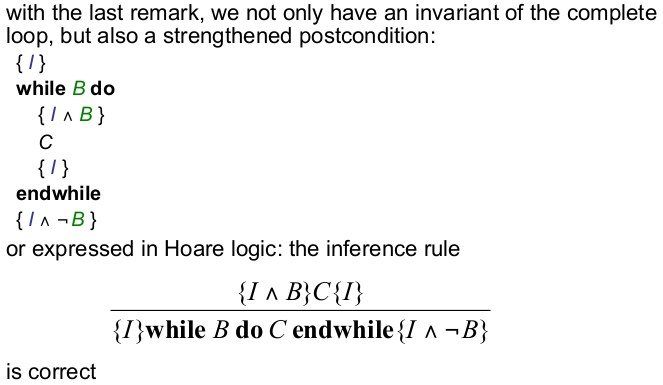
\includegraphics[width=0.7\textwidth]{figures/invariantLoop.png}
\caption{Invariants of a Loop}
\end{figure}

\hypertarget{finding-invariants}{%
\subsubsection{Finding Invariants}\label{finding-invariants}}

\begin{itemize}
\tightlist
\item
  to find an appropriate invariant is a creative process, just like
  programming
\item
  it cannot be automated
\item
  however, after having found an invariant, it can be added as
  annotation to the loop
\item
  and then, the generation of verification conditions can again be
  performed fully automatically
\end{itemize}

\clearpage